\subsection{Dynamical Reputation model}

\subsection{Selection of dynamical reputation model parameters} \label{section:param}
One of the largest drawbacks of DIBRM is the parameter tuning problem. In previous applications of the model \cite{melnikovDynamicInteractionBasedReputation2018,yashkina2020} there was no single best set of parameter values for modeling dynamic reputation in Stack Exchange communities. For example, in \cite{yashkina2020} the best approximation of the official Stack Exchange reputation is obtained with $t_a =2, \beta = 1, \alpha = 1.4$ which means there is no active forgetting factor. In our application of DIBRM to SE communities we opted for a different set of parameter values. Details of parameter search and tuning are presented in SI.

For basic reputation contribution of a single interaction we selected $I_{bn} = 1$ and at the same time this is the threshold value of an active user. This value is intuitive as every interaction has initial contribution of +1 to user's reputation, although the previous works have used values of +2 and +4. Following the previous work and after examining the median/average time between subsequent interactions of the same user, we selected $t_a = 1$, which also means that reputation in our model will be updated every day during the time-window of the analysis, regardless of whether the user is active or not. To emphasize the bursts of activity and frequent recent interactions, cumulative factor has a larger value $\alpha = 2$. Finally, the most delicate parameter is the forgetting factor, which at the same time determines the weight of past interactions and the reputational punishment due to user inactivity. Here we need to select the value of parameter $\beta$ so we include the forgetting due to inactivity but not to penalize is too much. In Fig. A1 we show how different values of parameter $\beta$ influence the time needed for user's reputation to fall on value $I_{n}=1$ due to user's inactivity and value of dynamical reputation in the moment of the last activity. The higher the value of parameter $\beta$ and initial dynamical reputation of users, the longer time it takes for user's reputation to fall on baseline value. For parameter $\beta=0.9$ and $I_{n}=5$, user's reputation falls on value $I_{n}=1$ after less than 20 days, while this time is doubled for $\beta=0.96$. We see, that for higher values of parameter $\beta$ the time needed for $I_{n}$ to fall on value $1$ becomes longer, and that the the initial value of reputation becomes less important. 

Figure A2 in SI shows the difference between the number of users that had at least one activity in the window of 30 days and number of users with reputation higher than $1$ during the same period for different values of parameter $\beta$. The minimal difference between these two variables is observed for the values of $\beta$ between $0.94$ and $0.96$ for both live and closed communities. Since we want to compare communities, we select $\beta = 0.96$ after verifying that this level of reputational decay does not reduce the number of active users (based on their dynamic reputation) below the actual number of users who have been active (interacted with the community) in the time window of 30 days. 

To summarize, our model of dynamical reputation has three parameters: 1) basic reputation contribution $I_{bn}=1$; 2) cumulative factor $\alpha=2$; 3) forgetting factor $\beta=0.96$. The selected values of parameters are used for measuring dynamical reputation of user in all four pair SE communities. Given these values of parameters, the minimal reputation achieved by the user immediately after they have made an interaction in the SE community is $1$. This reputation will decay below $1$ if the user does not perform another interaction within the one-day time window. For any user in a community, when their reputation drops below $1$, we consider this user inactive which means that the user at that time is not "visible" in the community and their past contributions at that time are unlikely to impact other users. The number of active users and mean user reputation for different Stack Exchange communities are shown in Fig. \ref{fig:dr6panel}.

\subsection{Dynamic reputation - $\beta$ parameter}

Our implementation of dynamic reputation model was based on $\beta = 0.96$. There are several reasons for selecting this value.

In Dynamic reputation model, the $\beta$ parameter controls the strength of the forgetting fator of the model.  The value of this parameter should reflect the core feature of the reputational systems and make reputation easier to loose. Due to user's inactivity, any level of reputation will eventually decay to below 1. Dependence of time needed for reputation to drop below this level and the $\beta$ parameter, as well as reputation before inactivity is shown on Figure~\ref{fig:betadelta}. Here $I_n$ is equal to the raw number of interactions in the community without forgetting or cumulative factor at work.

\begin{figure}[h!]
	\centering
	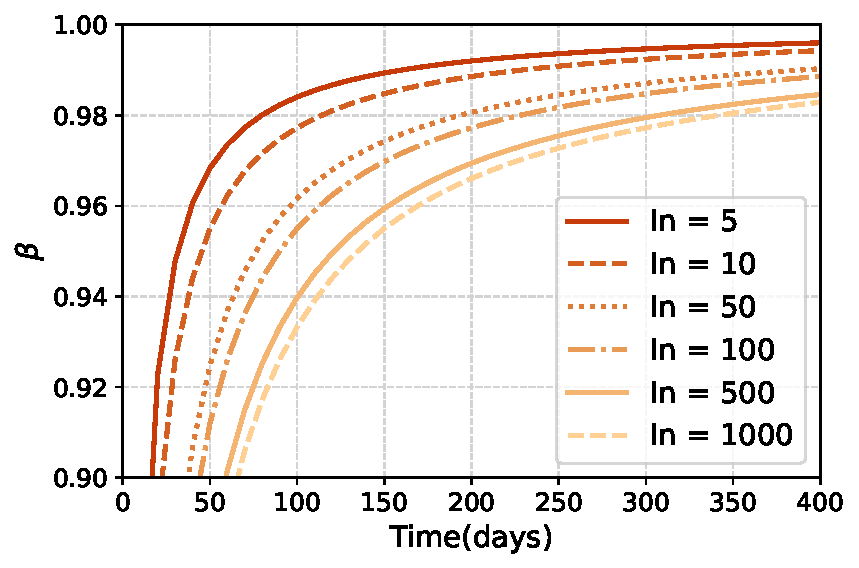
\includegraphics[width=0.5\linewidth]{figures/stackexchange/reputation_decay.pdf}
	% REMOVE 'SLOWER' FROM THE PLOT TITLE > zamenjeno i formulu sam prebacila u caption
	\caption{Dependence of parameter $\beta$ and number of days $\Delta$ needed for reputation $I_n$ to drop to $I_{n_0} = 1$. Dependence of parameter $\beta$ and number of days when reputation due inactivity decreases from $I_n$ to $I_0$ is given as  $\beta = (\frac{I_{n0}}{I_{n}})^{(1/\Delta)}$ }
	\label{fig:betadelta}
\end{figure}

\begin{figure}[h!]
	\centering
	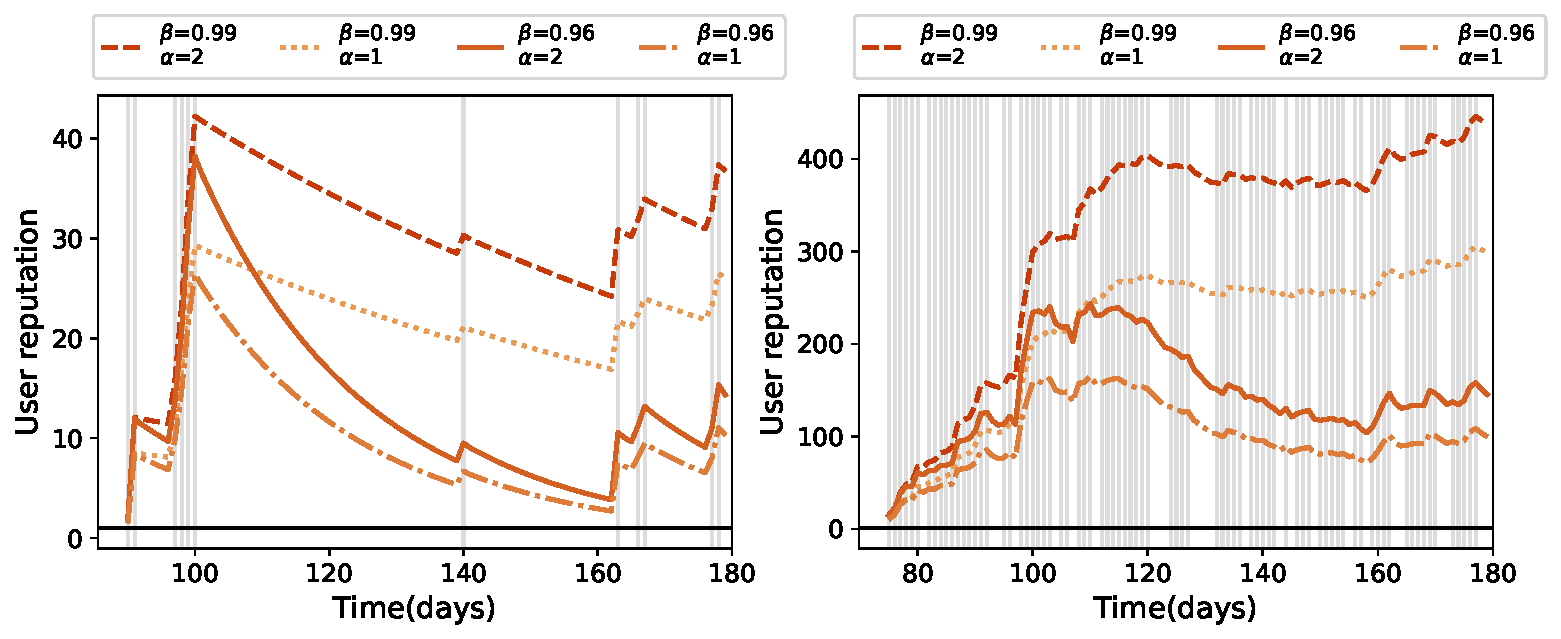
\includegraphics[width=\linewidth]{figures/stackexchange/single_user_reputation.pdf}
	% REMOVE 'SLOWER' FROM THE PLOT TITLE > zamenjeno i formulu sam prebacila u caption
	\caption{Single users reputations }
	\label{fig:singleuser}
\end{figure}

For $\beta$ values below 0.96, the decay is fast and within two to four months of inactivity even high values of reputation are reduced below the threshold. On the other hand, with $\beta$ values the decay proces is more differentiated and high reputation becomes harder to loose, surviving up to a year of inactivity. For $\beta$ equal to 0.96, it takes a month for reputation based on 5 interactions to decay and around five months for high reputation based on 500 or 1000 interactions to decay below the threshold.

\textbf{30 days sliding window} We compared the number of users with estimated reputation higher than 1 for different parameters $\beta$ and concluded that $\beta$ close to $0.96$ approximates the number of users with recorded interactions in a given 30 days sliding window. For each pair of communities we calculated number of users with at least one interactions in every 30 days sliding window and then we estimated several times series expressing the number of users with reputation higher than 1 for fixed $\beta$. Then we calculated the root mean square error (RMSE) between those time series for the first 200 days. Values of RMSE are shown on Figure~\ref{fig:rmse}. For each community, we can find parameter $\beta$ that minimizes RMSE. Although $\beta$ does not have a unique value across communities, it varies between 0.95 and 0.96. 
%We should notice that taking different time period, for example, the first 90 days, we can get different optimal values of betta, but they'll probably take values between 0.95 and 0.96 (I can test it). 


\begin{figure}[h!]
	\centering
	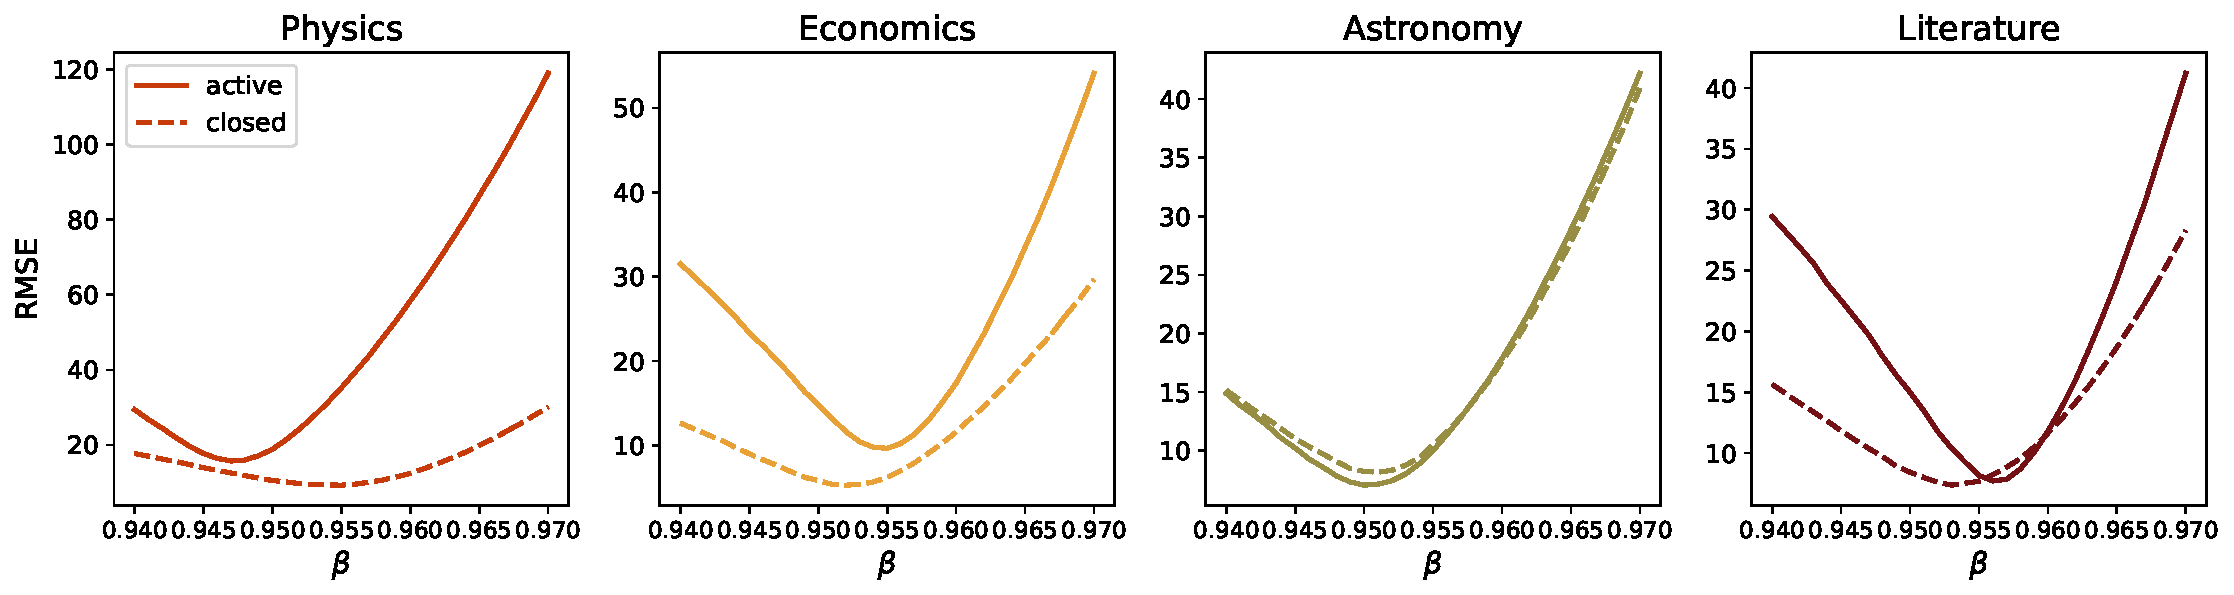
\includegraphics[width=\linewidth]{figures/stackexchange/rmse.pdf}
	\caption{RMSE between number of active users in sliding window of 30 days and number of users with reputation $>1$ for  $0.94< \beta <0.97$ with step $0.001$. }
	\label{fig:rmse}
\end{figure}

Figure \ref{fig:nusers} shows comparison between number of users in 30 days sliding window, number of users for these optimal values $\beta = 0.954$ and $\beta =0.96$. For $\beta = 0.96$ we observe that in most communities estimated number of active users consistently slightly higher than the actual number of users which have made at least one interaction in that sliding window. This means that dynamic reputation model in some cases overestimates the reputation of the user, but far more important is that it never understimates the real number of active users. Since we base our calculations of total and average reputation within the community only on users whose reputation is higher than the threshold this is important as no active users are disregarded by the model due to the value of the decay parameter.

\begin{figure}[h!]
	\centering
	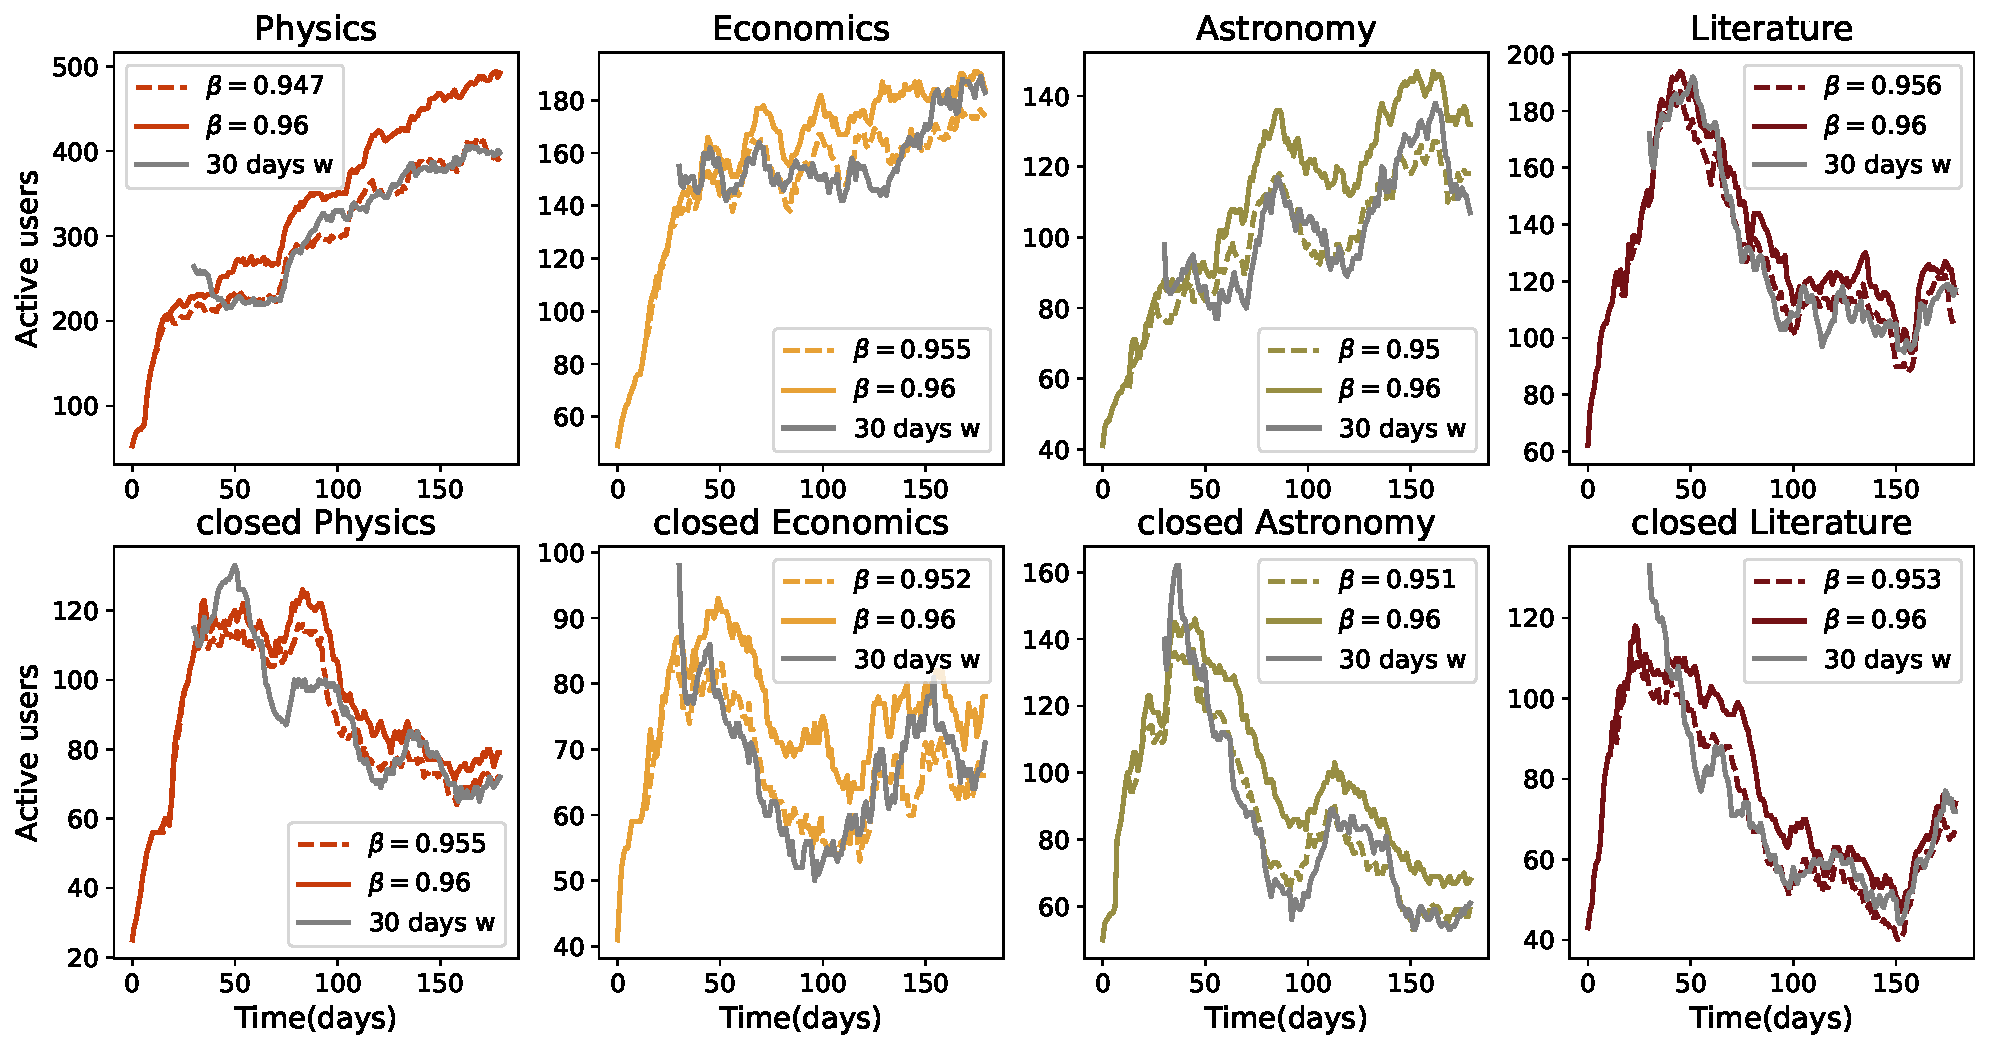
\includegraphics[width=\linewidth]{figures/stackexchange/active_users.pdf}
	\caption{Number of active users in a sliding window of 30 days and number of users with dynamic reputation higher than 1 for $\beta=0.954$ and $\beta=0.96 $ which provide the best fit to the number of users in 30 days sub-networks for each community}
	\label{fig:nusers}
\end{figure}

Finally, it's imporant that our dynamic reptuation captures the trend of long-term user activity. In Figure~\ref{fig:active-users} solid lines show the time series of estimated dynamic reputation for $\beta = 0.96$ while dashed lines show the number of users who were active in a given sliding window and continued to be active in the next one. Although the total estimated number of active users is expectedly higher, two time series follow similar trends in different communities.

\begin{figure}[h!]
	\centering
	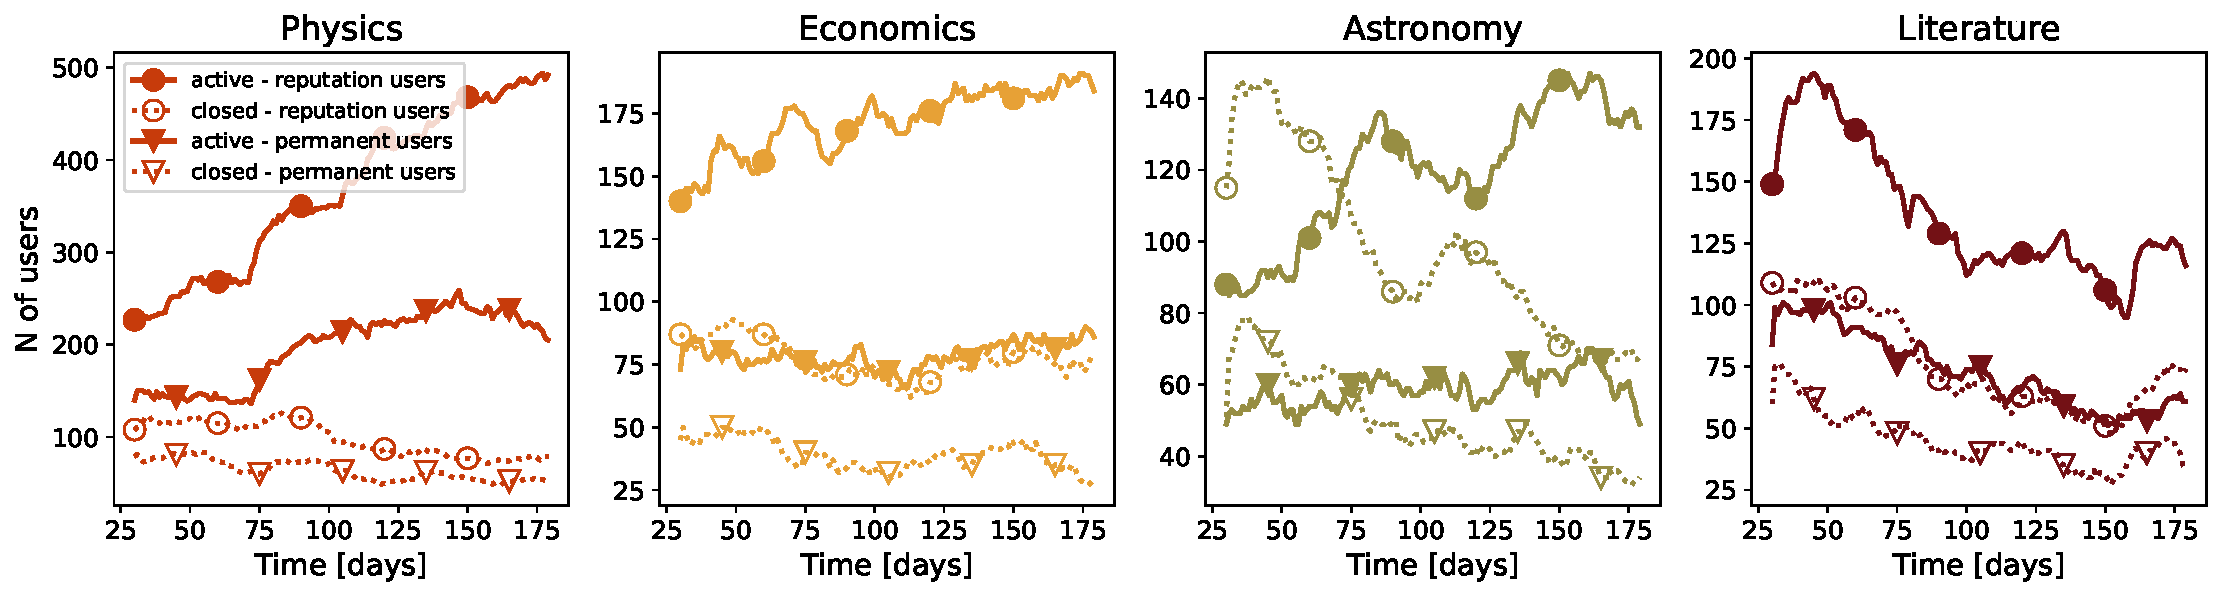
\includegraphics[width=1\linewidth]{figures/stackexchange/permanent_users.pdf}
	\caption{Solid lines represent number of users with dynamic reputation higher than 1 for $\beta=0.96$ while dashed lines are number of users within 30 days sliding window who were active and remained to be active. Blue lines are beta, while red lines are area51 communities.}
	\label{fig:active-users}
\end{figure}
\clearpage




\subsection{Dynamic reputation of users within the network of interactions}

\begin{figure}
	%%% 6 panels
	%%% columns: Total rep., Mean rep., Number of Active Users
	%%% rows 1: Physics. Theo. Physics, Econ. Beta, Econ. A51
	%%% rows 2: Astro Beta, Astro A51, Lit Beta, Lit A51
	\centering
	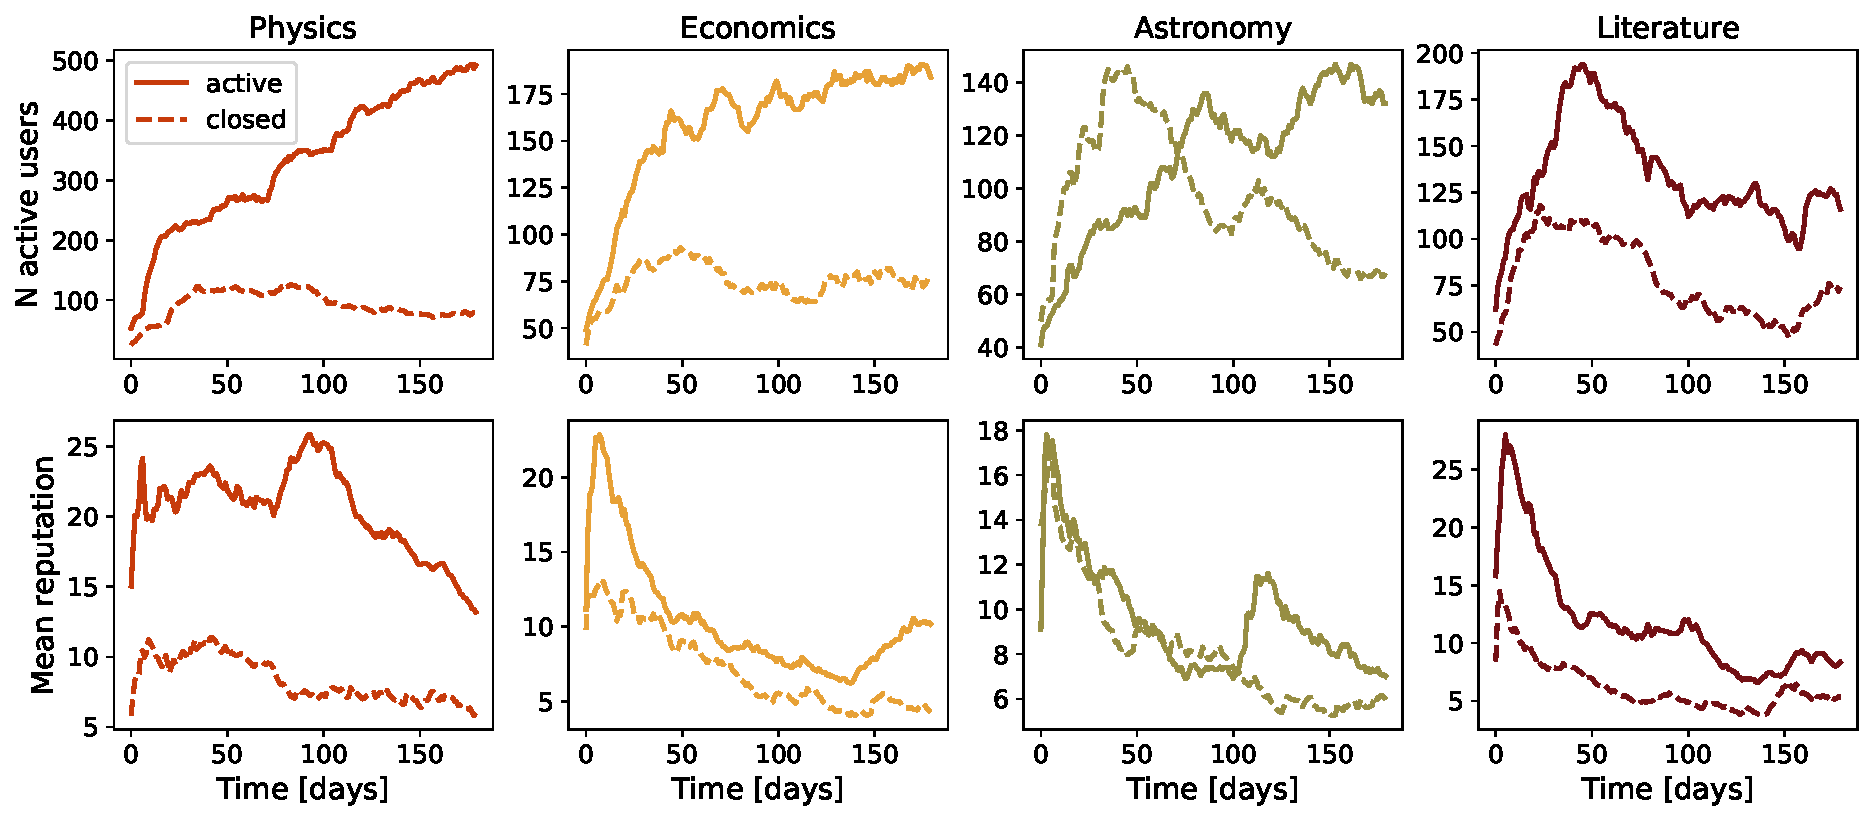
\includegraphics[width=\linewidth]{figures/stackexchange/reputation.pdf}
	\caption{Dynamic Reputation on the four pairs of Stack Exchange websites: Astronomy, Literature, Economics,  Physics and Theoretical Physics.}
	\label{fig:dr6panel}
\end{figure}

\begin{figure}
	\centering
	%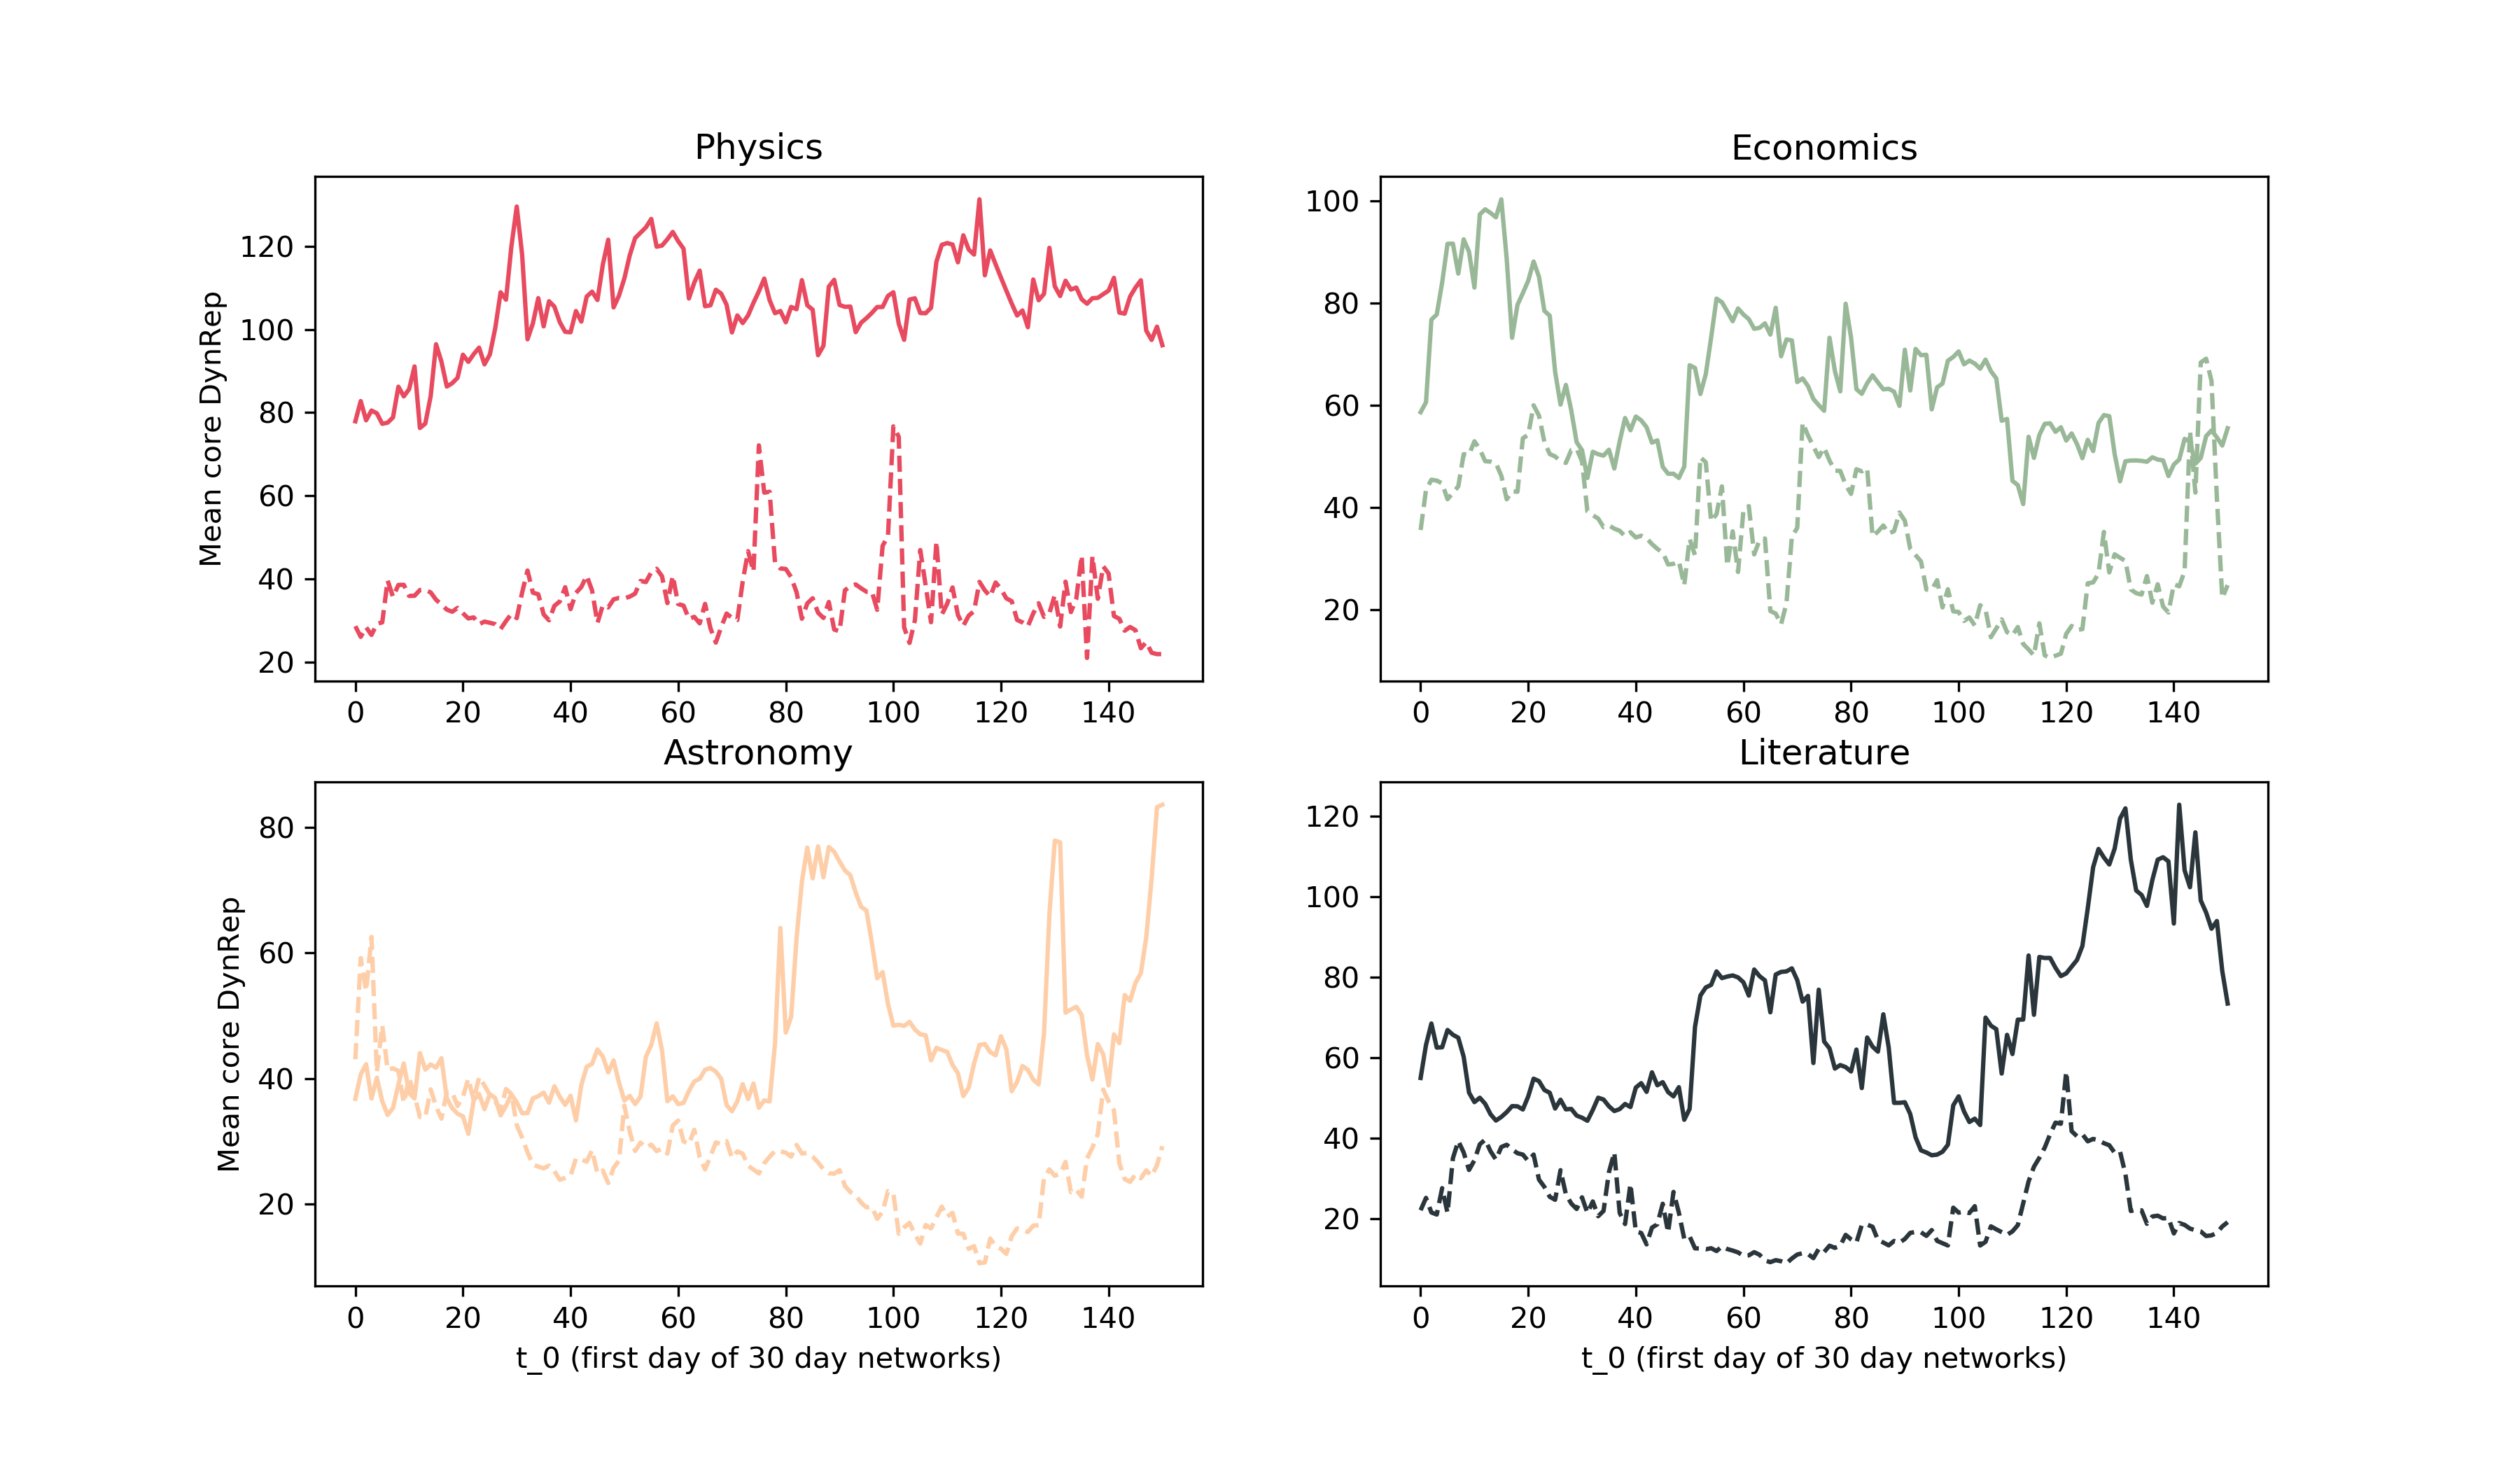
\includegraphics[width=\linewidth]{figures/Mean_core_dyn_rep.png}
	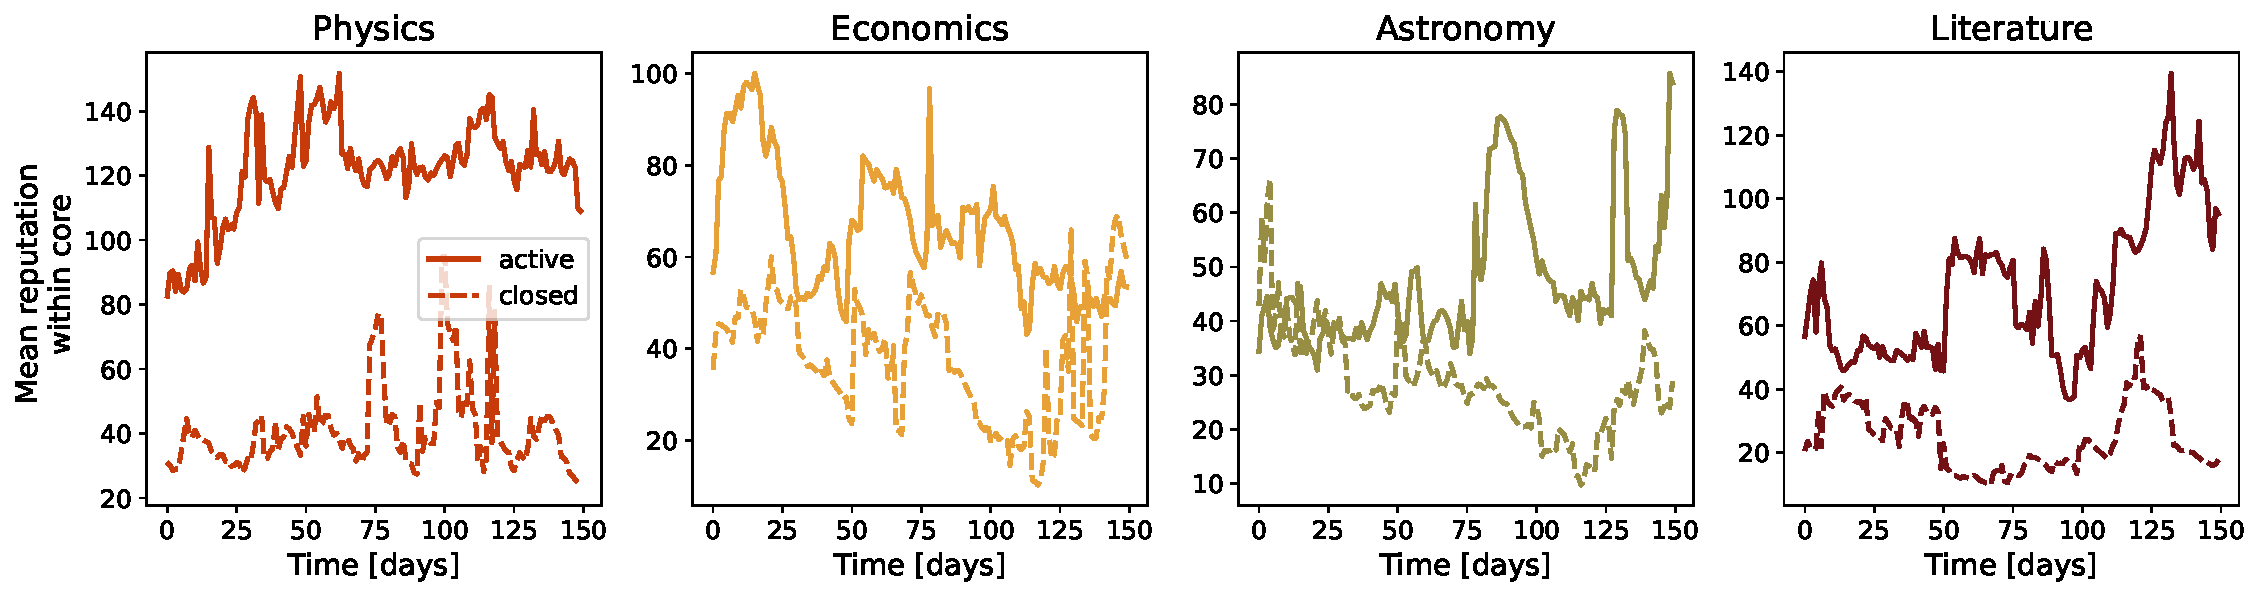
\includegraphics[width=\linewidth]{figures/stackexchange/core_reputation.pdf}
	\caption{Dynamical reputation within core.}
	\label{fig:dr_core}
\end{figure}

Examined network properties suggest that there are structural differences between active and closed communities. Active communities have higher and more stable local cohesiveness compared to their closed counterparts. The overlap of the set of nodes in the core for active communities shows a significant overlap even for distant subnetworks, meaning that the membership of the core in active communities is more stable.

To further explore the differences between active and closed communities, we focus on dynamical reputation which is our proxy for collective trust in these communities. We investigate whether and how core-periphery structure is related to collective trust in the network. Figure \ref{fig:dr_core} shows the mean dynamical reputation in the core of active and closed communities and its evolution during the observation period. There are clear differences between active and closed communities when it comes to dynamical reputation. The mean dynamical reputation of core users is always higher in active communities than in closed. As expected, the largest difference is observed between Physics and Theoretical Physics community. The difference between active communities which are still in the beta phase and their closed counterparts is not as prominent, however, the active communities have higher mean dynamical reputation especially in the later phase of community life. The only difference in the pattern is observed for astronomy communities at the early phase of their life, when closed community has a higher value of dynamical reputation than active community. This is in line with similar patterns in the evolution of mean clustering and core-periphery structure. 

By definition, the core consists of very active individuals and thus we expect higher total dynamical reputation of users in the core in comparison to the the total reputation of users belonging to subnetworks periphery. Figure A12 shows the ratio between the total reputation of core and periphery for closed and active communities and its evolution. The ratio between total reputation of core and periphery in Physics is always higher than in the Theoretical physics community. Similar pattern can be observed for literature communities, although the difference is not as clear as in the case of physics. Ratio of total dynamical reputation between core and periphery is higher for closed community than active one on the economics topic in the early days of community life. However, in the later stage of their lives this ratio becomes higher for active communities. Communities around astronomy topic deviate from this pattern, which once again shows the specificity of these communities. 

To complete the description of the evolution of dynamic reputation active and closed communities, we examine the evolution of Gini index of dynamical reputation in the whole network which is shown in Fig. A5 in Supplementary Information. The Gini index is always higher for active communities than for closed ones, especially for later times in observation period. Only pattern of Astronomy communities deviates from the pattern observed for other three pairs during the early days. These results indicate that the dynamical reputation is distributed in the population more unequally in the active than in closed communities. The evolution of assortativity coefficient that measures correlations between dynamical reputation of connected users in the subnetworks, shown in Fig. A6, shows that networks are disassortative for the largest part of the observation period. These results suggest that users with high dynamical reputation have tendency to connect with users with low value of dynamical reputation. 


In Figure~\ref{fig:dyn_rep_coreper} we show mean user reputation in core and in periphery over time (30 day sliding windows as before). We see that the mean user reputation in core is greater in the currently active sites (solid lines, top panels) than in their closed pairs (dashed lines). In the bottom panels, we see that the mean reputation on the network periphery has substantially lower values, and the difference between active and closed sites is less pronounced. 

For reference in Fig~\ref{fig:core_size} we show core sizes in all sites. We show these in absolute numbers (total number of nodes) and as a fraction of network size through time.






\textbf{Gini coefficient}
Besides the number of active users (who at given moment of observation have reputation higher than the threshold) and the population mean value of dynamical reptuation, we have investigated in more details the distribution of dynamical reputation within discussed communities. We have observed that the distributions are often skewed which prompted us to compare the communities in terms of their Gini coefficient. The gini coefficient is a simple measure that shows us the degree of reputation inequality within the community. We calculate the value based on the dynamic reputation values of users at every time step (day) and report he values in Fig.~\ref{fig:dynrep-gini}. We see that all communities (both still active and closed ones) have gini coeffiecinet values higher than $0.5$ throughout first six month period. Interestingly, except in the case of Astronomy, currently active communities had higher reputation inequality every day during first six month period. As in many other measures, in the case of astronomy, closed community started as more unequal one (signalled by higher gini coef values), but after around two months the situation changed. 
\begin{figure}[h!]
	\centering
	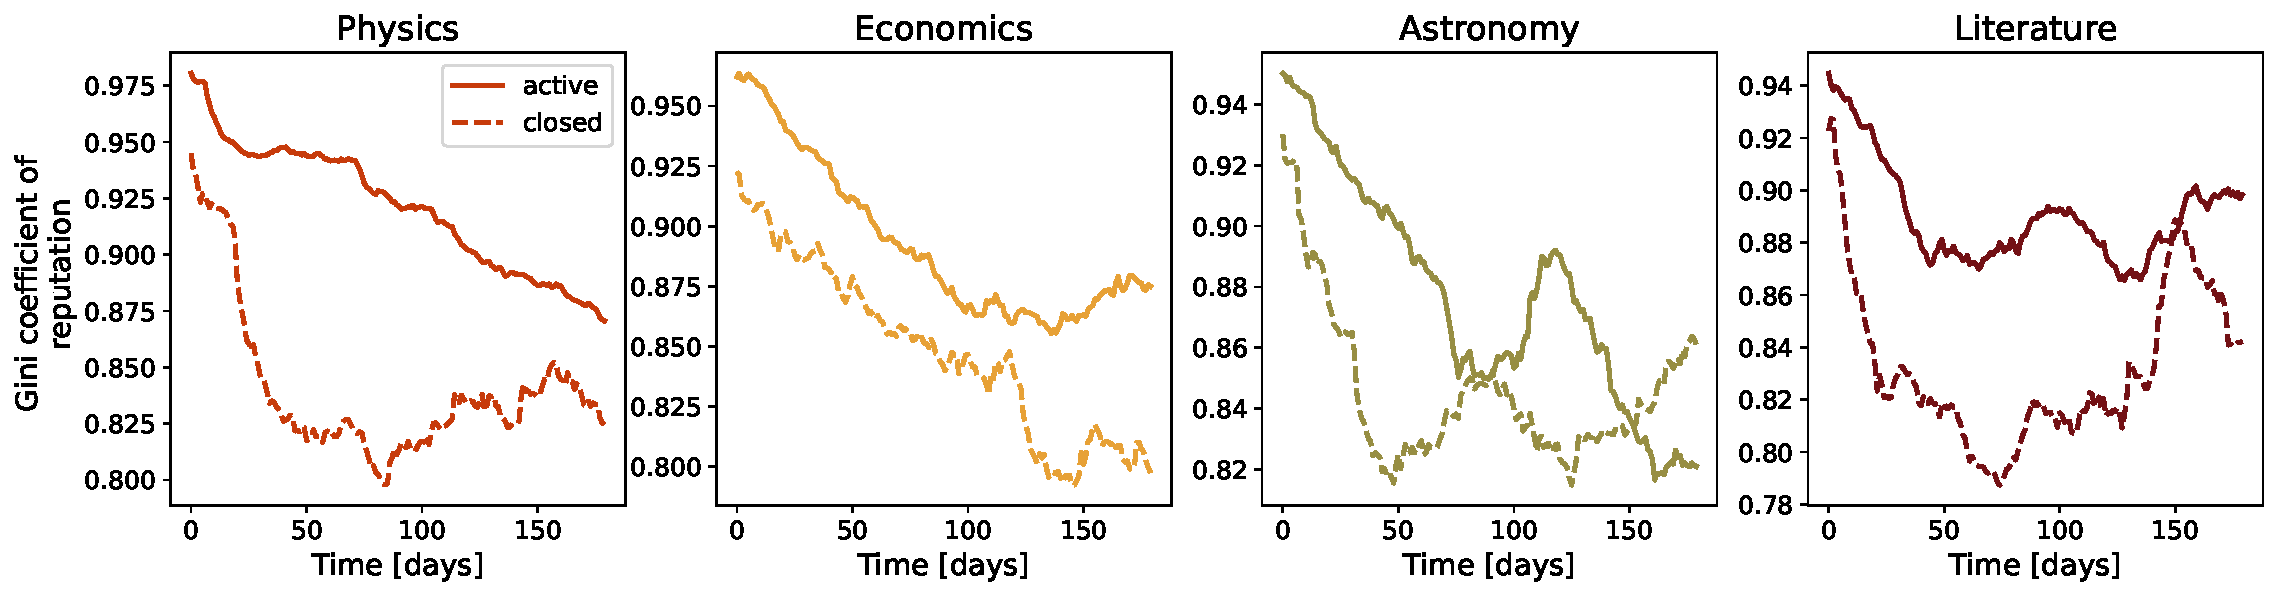
\includegraphics[width=1\linewidth]{figures/stackexchange/gini.pdf}
	\caption{Gini index of dynamic reputation within population}
	\label{fig:dynrep-gini}
\end{figure}

\subsection{Dynamic reputation in the network of interactions}
In the few figures below, we investigate whether users' dynamic reputation is related with users' position within the network.

\textbf{Dynamic Reputation assortativity}

We first look at user interaction patters, e.g. we investigate whether users connect with others of similar or different reputation (positive/negative assortativity). We operationalize this by measuring assortativity of dynamic reputation on interaction network. Practically this is a meassure of correlation between dynamic reputation of users who are linked in the interaction network. These results are shown in Fig.~\ref{fig:dyn_rep_assort}. We look at 30 day unweighted undirected networks of interactions (questions, answers and comments) and calculate assortativity by using users' reputation on the last day of observed time window. We see small values of assortativity that are mostly negative, signaling weak correlations between reputation levels of interacting users. The fact that the values are mostly negative are expected, users of different dynamic reputation interact, e.g. active, high reputation users respond to the questions of new, less reputable users. Exceptions are closed astronomy and literature sites that occasionally had positive assortativity values, signaling existence of links between users of similar reputation levels.
\begin{figure}[h!]
	\centering
	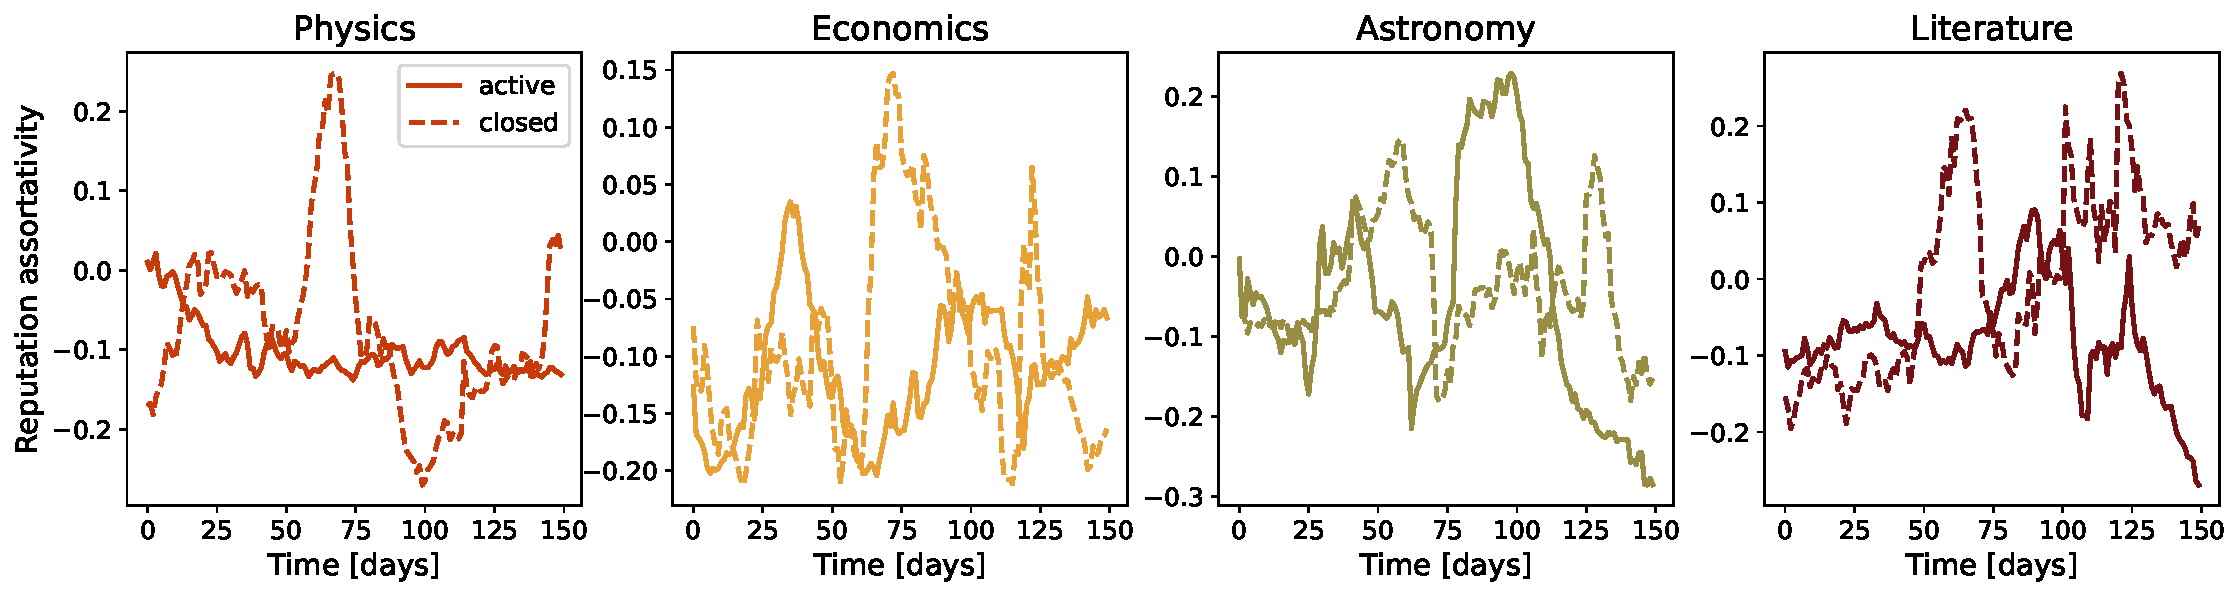
\includegraphics[width=1\linewidth]{figures/stackexchange/reputation_assortativity.pdf}
	\caption{Dynamic Reputation assortativity in the network of interactions (questions, answers, comments, unweighted, undirected network). Solid lines - active sites; dashed lines - closed sites.}
	\label{fig:dyn_rep_assort}
\end{figure}
%% posto se ovo isto gleda na mrezama mozda moze u isti section sa ova dva grafika
\\~\\
\textbf{DynRep \& Degree}
% dodacu samo korelacije kroz vreme za sad stoji samo placeholder za sliku i opis
\textbf{DynRep \& BC}
% dodacu samo korelacije kroz vreme

We continue to investigate whether the user's reputation correlates with typical network centrality measures calculated at user's node in the interaction network. As previously, we compare node's centrality in the 30 day network with the node's dynamic reputation on the last day of the period, repeat the process every day for the first six months. 
Correlation coefficient between dynamic reputation and degree in the network is very high, as expected, as most of the interactions that contributed to user's reputation are also present as links in the network. We show these results in Fig.~\ref{fig:dyn_rep_centrality}(top). However, we again see the distinction between active and closed communities where this correlation is higher in active communities, except in the first month of sliding windows. Astronomy is an exception here as well as we see that the correlations were similar in both closed and still active sites throughout observed period. 
%There are few steep drops in correlation coefficients in Economics and Literature closed sites, maybe worth further investigation.
In the bottom panels of Fig.~\ref{fig:dyn_rep_centrality} we present correlation coefficients of dynamic reputation and user's betweenness centrality in the interaction network. These corrlations are also high and most of the time higher in the later networks of active than closed communities. This is particularly interesting due to global nature of betweenness centrality measure and less obvious relation of it to user's dynamic reputation.
\begin{figure}[h!]
	\centering
	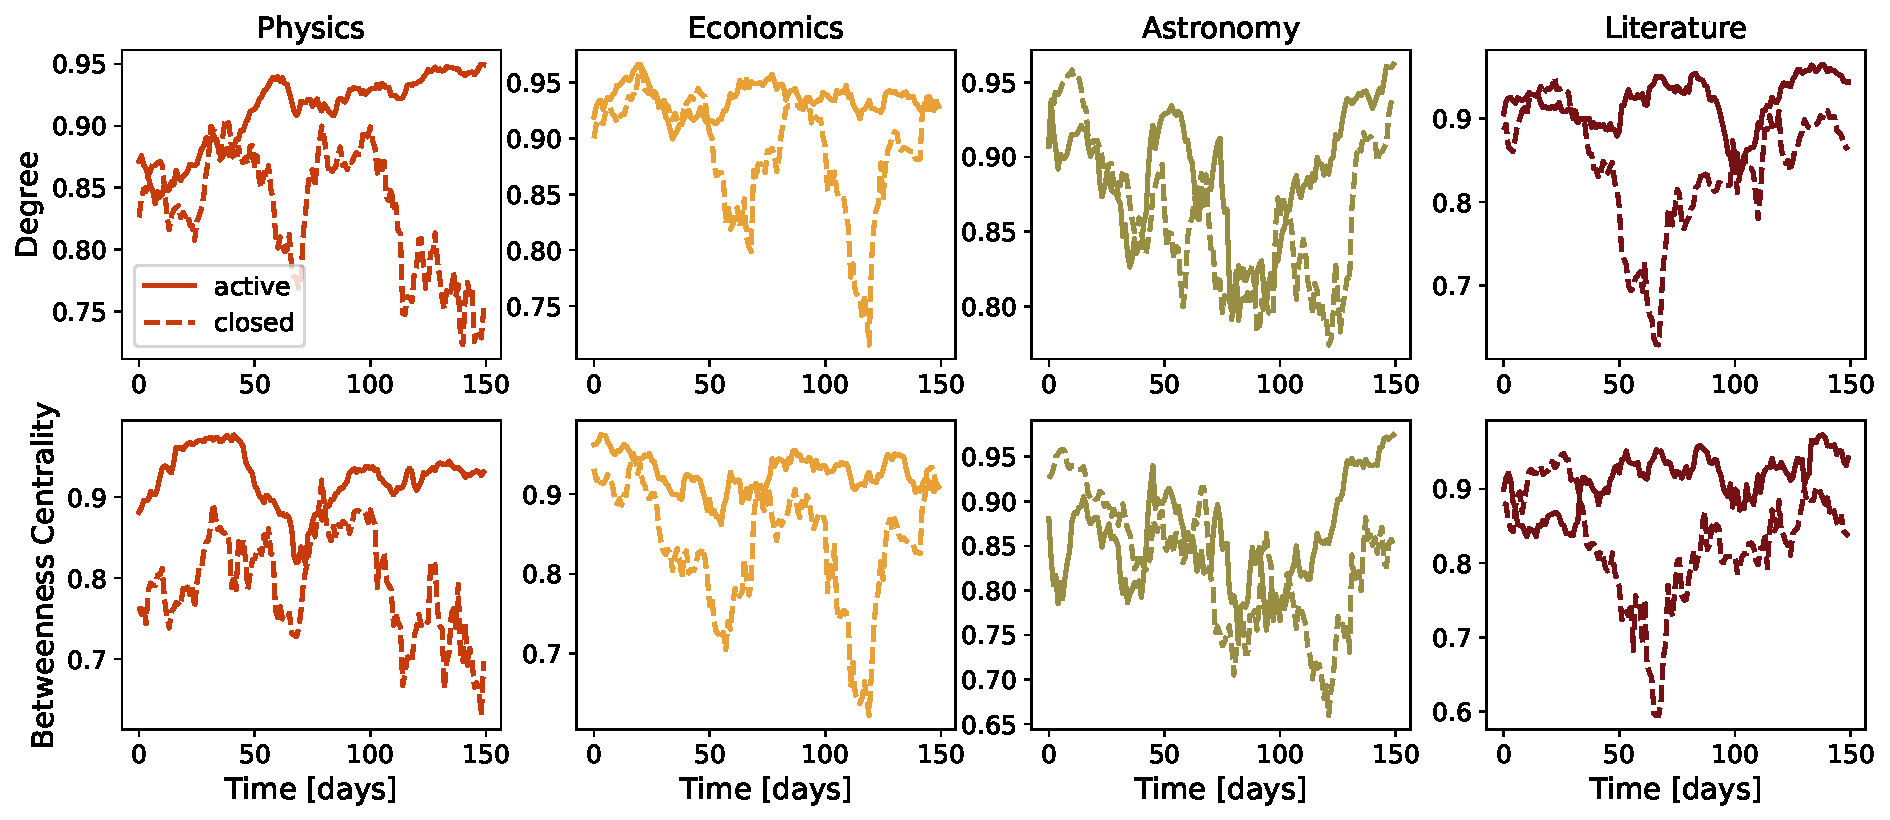
\includegraphics[width=\linewidth]{figures/stackexchange/correlations.pdf}
	\caption{Coefficient of correlation between users' Dynamic Reputation and users' network degree (top) and users's betweenness centrality (bottom). Solid lines - active sites; dashed lines - closed sites.}
	\label{fig:dyn_rep_centrality}
\end{figure}





       
